\chapter{Work Description}
\label{cap:descripcionTrabajo}

\section{Style Analyser}
In order to generate messages with the user's writing style, it is necessary to define parameters which will determine and describe it. For this purpose, we have developed a style analyser that extracts the messages written by the user and obtains the value of various metrics from them. Then it will be useful for analysing different user's emails and drawing conclusions about what parameters describe the writing style of each person more accurately. Besides most of the developed code will be reusable in the final application for analysing the user's messages.

In this section we are going to explain the architecture of this analyser (see \ref{ssection:stylearch}) and each of the modules that compose it (they are explained in sections \ref{ssection:extmod}, \ref{ssection:prepmod}, \ref{ssection:typomod} and \ref{ssection:measmod}). Finally, we are going to discuss the obtained results and analyse them for drawing a conclusion (this discussion can be looked up in \ref{ssection:resconc}).

\subsection{Architecture} \label{ssection:stylearch}
The first step when we are designing a system's architecture is to know its input and output. In this case, we want to implement a natural language processing system that analyses the writing style of emails. As we have previously mentioned, the writing style analysis will be represented through chosen metrics. Therefore, our system's output is going to be that chosen metrics (they are explained in section \ref{ssection:measmod}).

In respect of the system's input, because of the nature of the problem we face, it is reasonable to think that it must be a single email. However, we do not have the corpus of emails to analyse. For this reason, our first step will be to extract the emails that will be analysed. Hence, our system's input is going to be the Gmail user for accessing to the information that we are interested in. Therefore, we are going to develop a system which receives a Gmail user as input and obtains different metrics of each message sent by the given user as output.

Once we clearly know the input and output of our system, we need to define the different steps that a message have to take for being analysed. In this way, we are going to design a pipeline architecture with four different phases (extraction, preprocess, typographic correction and measuring) as Figure \ref{fig:arch} shows. Thus, we divide the original job in 4 different and more simple tasks with distinct inputs and outputs required.

\begin{figure}[h]
	\centering%
	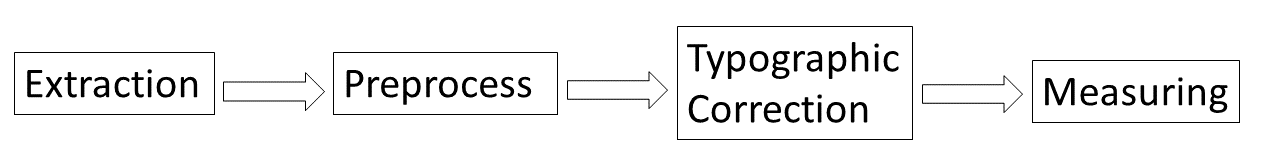
\includegraphics[width = 1\textwidth]{Imagenes/Bitmap/architecture.png}%
	\caption{Pipeline architecture of the style analyser}%
	\label{fig:arch}
\end{figure}

As it is easy to deduce, each of these phases is going to be developed as a different module. This implementation will have the advantage that each module is going to be able to work independently from the other modules, which will allow them to work in parallel. That is to say, while a message is being extracted, other e-mails could be being preprocessed, corrected or measured if they have gone through the previous phases.Let us now briefly explain what each of the defined phases consists of.

The first step, extraction phase, as the reader can imagine, consists of the extraction of each one of the sent messages of the given user. In this task, we are going to take advantage of all the studied concepts about the Gmail API (see Section \ref{ssect:gmailapi}) and make use of every resource it provides us. Besides, we will try to minimize the consumed quota units in each extraction, which means we will only make the requests to the Google Servers that are strictly necessary. This first step is not just the task of extracting the resource that represents each sent message from the user's account, but also the job of transforming it to the format that the preprocessing module needs. Hence, the input of this module will be the same input as that of the complete system (a Gmail user) and its output will be an extracted message ready for being preprocessed.

As for the second step, the preprocessing phase, consists of the modifying the extracted message so that it can be interpreted by the natural language processing model to be used. Some of the changes that a message could suffer in this phase are: the removal of the signature, the disposal of the replied messages which appears under the text, the elimination of soft break lines that quoted-printable codification (see Section \ref{sssect:quot-p}) introduce in some messages, etc.

\subsection{Extracting Module} \label{ssection:extmod}

\subsection{Preprocessing Module} \label{ssection:prepmod}

\subsection{Typographic Correction Module} \label{ssection:typomod}

\subsection{Measuring module} \label{ssection:measmod}

\subsection{Results and conclusions} \label{ssection:resconc}
